\section{Conclusion and a critical evaluation of the various algorithms}
\label{chap:Conclusion}

\quad \, After an exhaustive study of the various models and techniques, we are prepared to decide which method is most appropriate for each type of circumstance.\\

\begin{figure}[H]
\label{fig:scores1}
%\centering
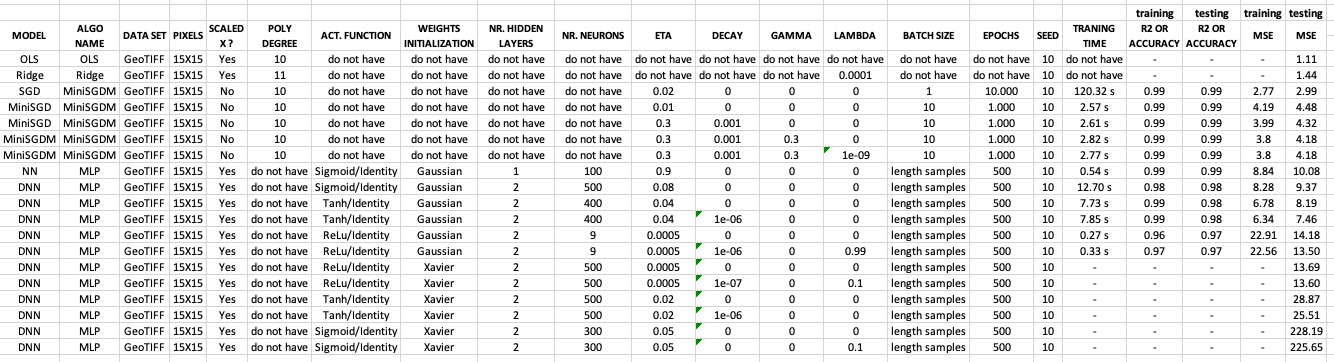
\includegraphics[width=16cm]{scores1}
\caption{Fitting different models and parameters, and assessing predictions for the GeoTIF image data.}
\end{figure}

Starting with the GeoTIF terrain data-set, the table above demonstrated that the Stochastic Gradient Descent (SGD) model presented the best MSE testing score of 2.99 among Gradient Descent (GD) and Neural Networks (NN) varieties. This score is pretty close to the ones achieved in the traditional methods of Ordinary Least Square (OLS) of 1.11 and Ridge Regression (RIDGE) of 1.44. However, the SGD model proves to be very inefficient in computation cost, as evidenced by the elapsed training time of 120 seconds. The other types of GD are quicker in terms of training but less accurate. Furthermore, the GD model's types might be more precise than the NN model's diversities because the former applies a polynomial transformation on its input data, likewise OLS and RIDGE, while the latter uses random numbers between 0 and 1. The NN species' most significant benefit is that the descriptive data does not need a polynomial transformation to feed the model.

\begin{figure}[H]
\label{fig:scores2}
%\centering
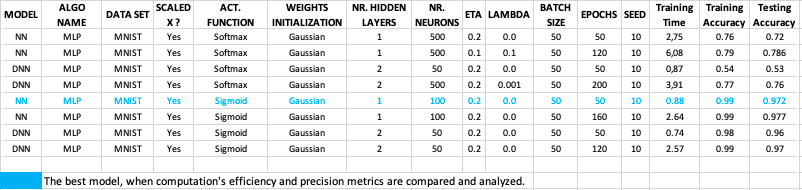
\includegraphics[width=16cm]{scores2}
\caption{Fitting different models and parameters, and assessing predictions for the MNIST data.}
\end{figure}

In its turn, the MNIST's results show that the Multi-Layer Perceptron (MLP) model using Sigmoid as the activation function and Accuracy-score as the cost function is more precise than Softmax with Accuracy-score. In fact, the handwriting images' predictions got an excellent testing accuracy of 97 percent with Sigmoid, while only 78 percent with Softmax. It is essential to state that an MLP model with Sigmoid and Accuracy-score resembles a Logistic Regression model, except that the former utilizes NN techniques as Mini-batch, Feed-Forward, and Back-Propagation, while the latter only uses Mini-batch and gradient descent.

\begin{figure}[H]
\label{fig:scores3}
%\centering
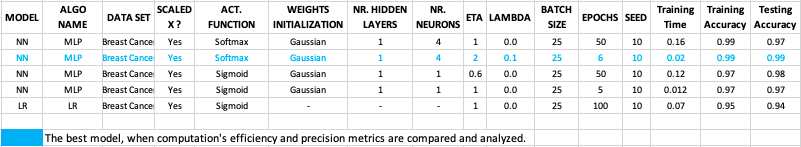
\includegraphics[width=16cm]{scores3}
\caption{Fitting different models and parameters, and assessing predictions for the Breast Cancer data.}
\end{figure}

Finally, the Breast Cancer outcomes reveal that the MLP model can predict cancer incidence in patients with an outstanding facility, precision, and efficiency. Actually, with only one hidden layer and as few as one neuron in this layer, the MLP with Sigmoid and Accuracy-score activation and cost functions, respectively, got the testing exactness metric of 97 percent. On the other hand, the MLP with Softmax and Accuracy-score activation and cost functions, respectively, got even better testing precision of 99 percent. Both models were rapid in their training, without any relevant difference. Regarding to the Logistic Regression method, it also proves to be very reliable and quick, although with less precision than NN models.\\

After all, one can conclude that the NN performed by MLP was more trustworthy for Classification than for Regression problems. However, NN and MLP are essential instruments to predict non-linear regression problems that can not be submitted to a polynomial transformation before fitting. Besides, NN models can achieve better results if applied with a larger number of hidden layers, neurons, and epochs. This study was restricted by two hidden layers and 500 epochs due to expensive computation cost, but a larger value for these parameters could have gotten more considerable metrics, which could be a good idea for future works.
